\documentclass[12pt,letterpaper,fleqn]{article}

%       amslatex provides nice math extensions for typesetting mathematics
\usepackage{amsmath}
\usepackage{amsfonts}
\usepackage{tmmaths}
\usepackage{sympytex}

%       pstricks provides powerful environments for incorporating postscript into a
%       TeX/LaTeX document. You must have a postscript printer and a package like
%       dvips to convert the DVI file to a PS file.
%\usepackage{pst-all}
%\usepackage{pstricks,pst-plot}
%\usepackage{pst-coil,pst-node}

%  This package provides native tex support for numbered grids. The syntax is:
%  \graphpaper[spc](x_lowleft,y_lowleft)(x_upperright,y_upperright)

%\usepackage{graphpap}
%\usepackage{float}

%  The package below must be initialized with "\initfloatingfigs" immediately after the
%  "\begin{document} command.
%\usepackage{floatfig}

\usepackage{graphicx}
\graphicspath{{i:/mytex/graphics}}
\DeclareGraphicsExtensions{.ps,.eps}

%       tst is a package for the creation of exams, quizzes and tests. the include
%       file mathstuf (see below) provides many abbreviations for these environments.
%\usepackage{tst}

%       epsfig is a package which provides for the inclusion of Encapsulated PostScript
%       files in a document.
%\usepackage{epsfig}
%\usepackage{epic,eepic}
\include{mathstuf}
\usepackage[total={7.25in,10in},top=0.25in,left=0.75in,includehead]{geometry}
\usepackage{fancyhdr}
\pagestyle{fancy}
\lhead{Math 252}
\rhead{\large Name\makebox[2in]{\hrulefill}}
\chead{\LARGE Exam 1, Make Up}
%\lfoot{\today}
\cfoot{}
%\rfoot{\thepage}
\renewcommand{\headrulewidth}{0.4pt}
\renewcommand{\footrulewidth}{0.4pt}
\setlength{\parindent}{0pt}
\setlength{\parskip}{2ex}

\newcounter{tf}[enumi]
\newenvironment{tf}[0]{\begin{list}%
{\alph{tf}. \makebox[5em]{True\hfill False}}%
{\usecounter{tf}\setlength{\labelwidth}{7em}%
\setlength{\leftmargin}{3.5cm}%
\setlength{\labelsep}{1cm}}}%
{\end{list}}

%\usepackage{epic,eepic}
\newcommand{\numline}{%
%\newcounter{mark}%
%\setcounter{mark}{-1}%
\setlength{\unitlength}{0.1in}%
\begin{picture}(0,0)%
\thicklines%
\put(0,0){\line(1,0){60}}%
\multiput(0,0)(10,0){7}{\line(0,-1){1}%
\makebox(0,-1.5)[t]{\arabic{mark}}\stepcounter{mark}}%
%
\thinlines%
\multiput(0,0)(5,0){12}{\line(0,-1){0.5}}%
\multiput(0,0)(1,0){60}{\line(0,-1){0.3}}%
%\put(-5,265){\makebox(0,0)[l]{{\bf cm}}}%
\end{picture}}%

\newcommand{\ds}{\displaystyle}
\usepackage{amsfonts}


\let\oldhat\hat
\renewcommand{\hat}[1]{\oldhat{\boldsymbol{\mathbf{#1}}}}
\newcommand{\lv}[1]{\ensuremath{\langle #1 \rangle}}
\renewcommand{\i}{\ensuremath{\hat{\imath}}}
\renewcommand{\j}{\ensuremath{\hat{\jmath}}}
\renewcommand{\k}{\ensuremath{\mathbf{\oldhat{k}}}}
\newcommand{\ora}[1]{\ensuremath{\overrightarrow{#1}}}
\renewcommand{\vec}[1]{\ensuremath{\mathbf{#1}}}
\renewcommand{\v}[1]{\ensuremath{\vec{#1}}}
\newcommand{\abs}[1]{\ensuremath{\lvert #1 \rvert}}

\usepackage{tabularx}
\usepackage{paralist}
\newcommand{\red}[1]{\textcolor{red}{#1}}
\newcommand{\blue}[1]{\textcolor{blue}{#1}}
% \newcommand{\ans}[1]{\quad\fbox{answer: \red{#1}}}
\newcommand{\ans}[1]{\mbox{{\bf Ans:} \blue{#1}}}
\newcommand{\dd}[2][]{\ensuremath{\frac{\text{d}#1}{\text{d}#2}}}
\newcommand{\eval}[2]{\ensuremath{\left.#1\right|_{#2}}}

\usepackage{amsthm}

\theoremstyle{definition}
\newtheorem*{definition}{Definition}

\usepackage{enumitem}
\usepackage{subfig}

\begin{document}
Do the problems below in a neat, clear and complete manner on the paper provided to you. If I am unable to follow your solutions, if enough detail is not provided, you will lose points.
\begin{enumerate}
 \item Set up and evaluate a definite integral to find the shaded area between the graphs of $y^2 - x = 3$ and $y - x = 1$ shown below. Hint: The answer is between 3 and 5 square units.
       \begin{figure}[!htb]
        \centering
        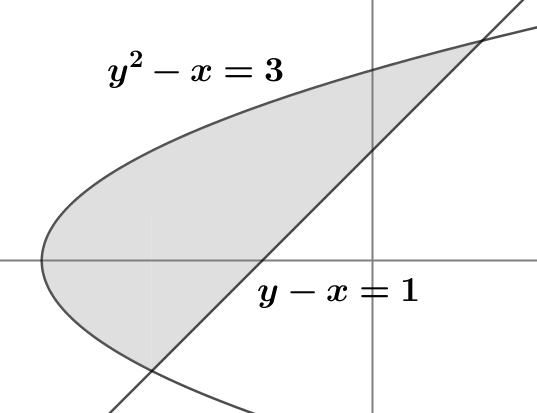
\includegraphics[width=0.4\textwidth]{img/area_between_graphs.png}
        % \caption{}
        % \label{}
       \end{figure}
 \item The temperature $T$ (in degrees Celsius) of a cup of coffee $t$ minutes after it is poured is given by the function
       \begin{equation*}
        T(t) = 20 + 75e^{-0.02t}
       \end{equation*}
       Set up and evaluate a definite integral to find the average temperature of the coffee over the first half-hour (30 minutes) after it is poured. Give your answer to the nearest degree. Hint: The answer is between 60 and 80 degrees Celsius.
 \item The region of the $xy$-plane bounded by the $x$-axis, the line $x = 2$ and the curve $y = \sqrt{x}$ is rotated about the line $x = -1$ to create a solid of revolution. Set up, but \emph{do not evaluate} definite integrals to find the volume of the solid using:
       \begin{enumerate}
        \item Cylindrical shells
        \item Rings (washers)
       \end{enumerate}
 \item A solid has the base shown on the left in the diagram below. Cross sections perpendicular to the base and $x$-axis are isosceles right triangles as shown on the right in the diagram. Set up and evaluate a definite integral to find the volume of the solid.
 \begin{figure}[!htb]
	\centering
	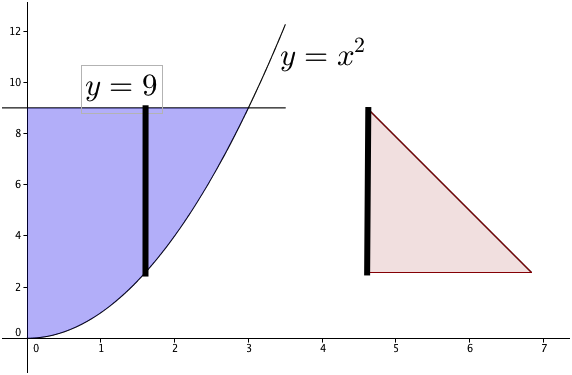
\includegraphics[width=0.5\textwidth]{img/Volume_of_solid.png}
	% \caption{}
	% \label{}
\end{figure}
 \item A 30 foot cable hangs over the edge of a 50 foot tall building. Its ``weight density'' (pounds per foot) is given by $\delta(y) = 5 - 0.1y$, where $y$ is the distance from the bottom of the cable; A small segment of cable of length $dy$ at location $y$ from the bottom of the cable weighs $\delta(y)\;dy$ pounds.\\[1.5ex] Set up and evaluate a definite integral to find the work done in pulling the cable up to the top of the building. Hint: The answer is between 1500 and 2000 ft-lbs.
\end{enumerate}
\end{document}
